\chapter{Background Estimation} \label{chapter:background}

\FloatBarrier
\section{Data-Driven Background Estimate}

    The basic event selection does not remove all non-signal events.
    Indeed, based on the relative rates of QCD multijet events (Figs. \ref{fig:lhc_rates} and \ref{fig:multijet_rates}) and the SM \vbfhhproc process (1.18 fb, see Table \ref{tab:mcyields}),
        most of the events remaining in the data are very likely background.
    Since these background events cannot be effectively differentiated from the signal,
        a technique must be used to estimate how much of the observed data are coming from background.
    Specifically, the analysis employs a method to predict the kinematic shape (in \mhh)
        of the background events within the 4b Signal Region,
        without directly observing that set of events.

    \begin{figure}[tbh]
        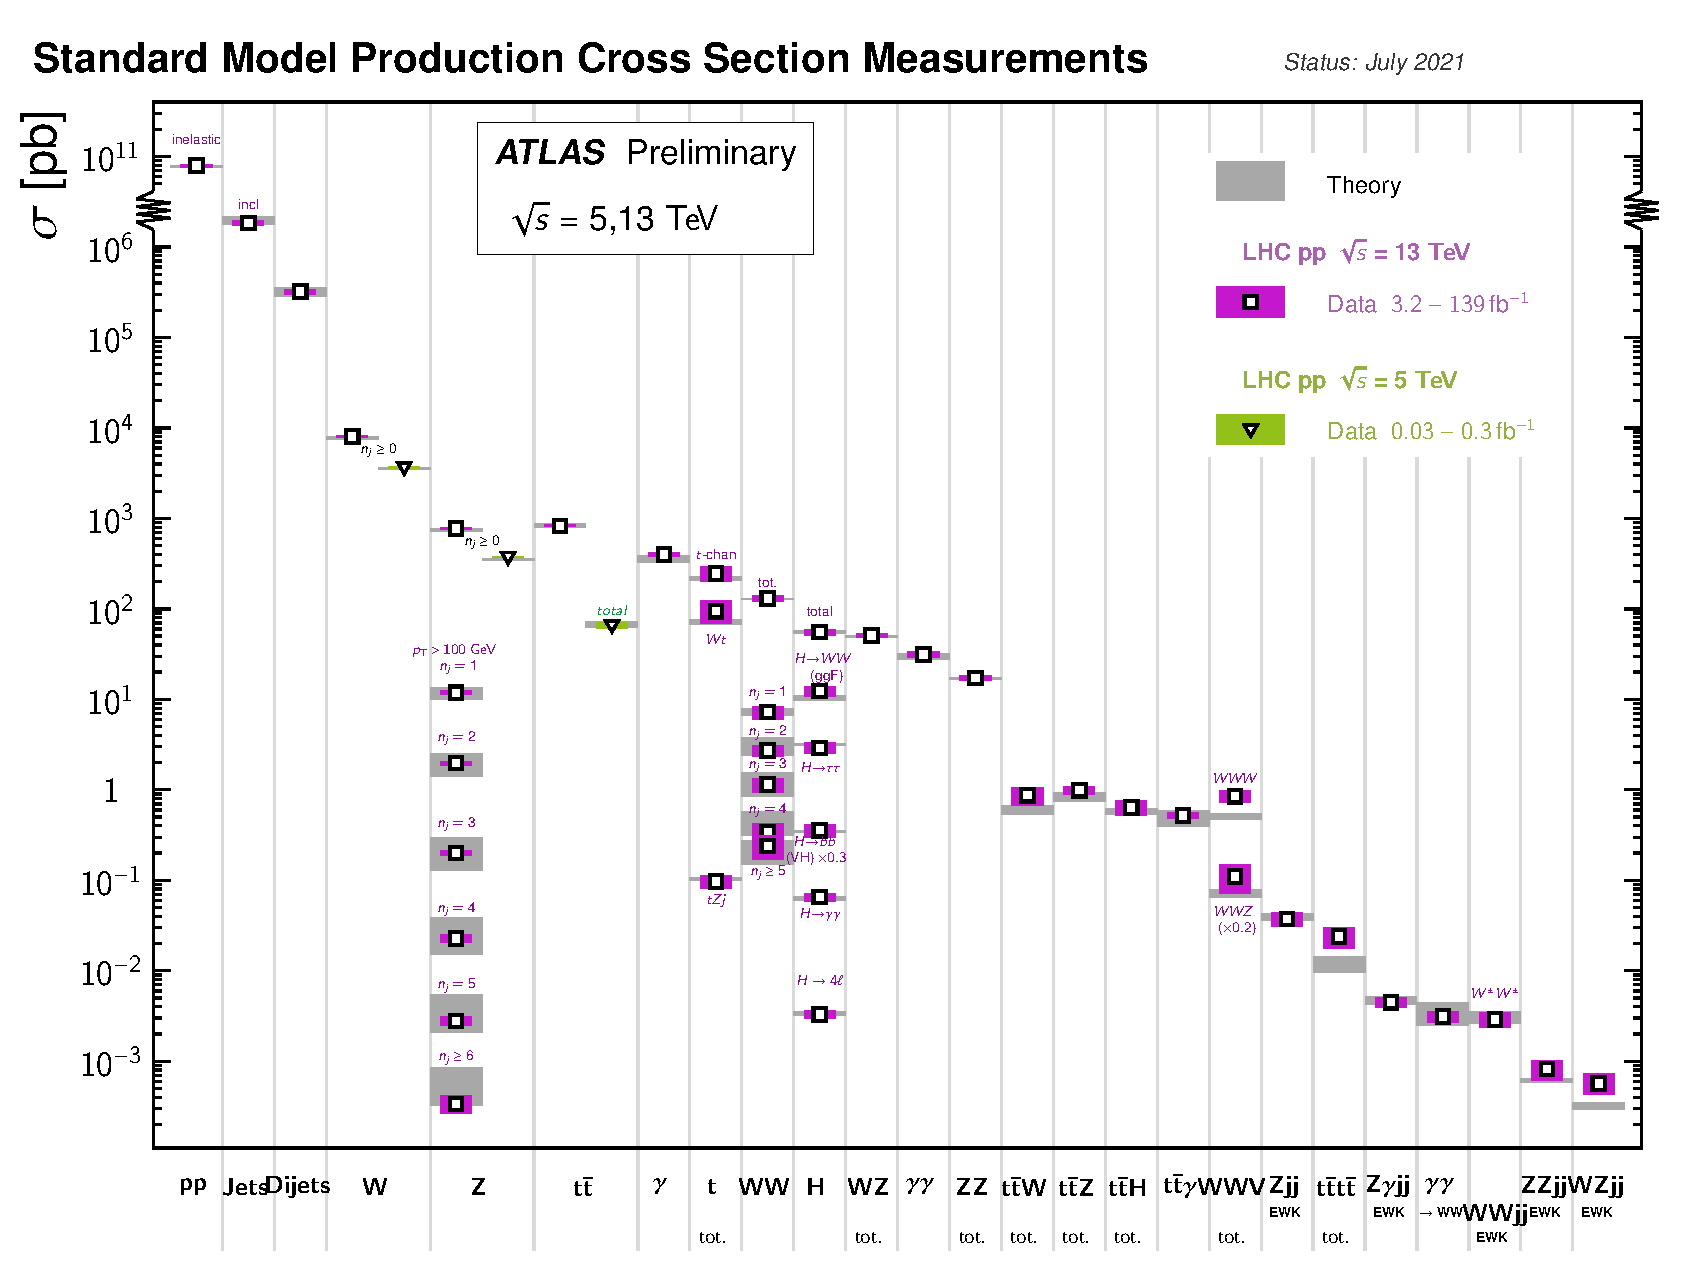
\includegraphics[width=\linewidth,height=\textheight,keepaspectratio]{background/lhc_rates}
        \caption{
            Production cross-section of various final states in ATLAS\cite{atlas_sm_summary}.
            Note the $\sim 1 \times 10^3$ pb cross-section of \ttbar events
                as compared to the 1.18 fb cross-section of the SM \vbfhhproc process.
        }
        \label{fig:lhc_rates}
    \end{figure}


    \begin{figure}[tbh]
        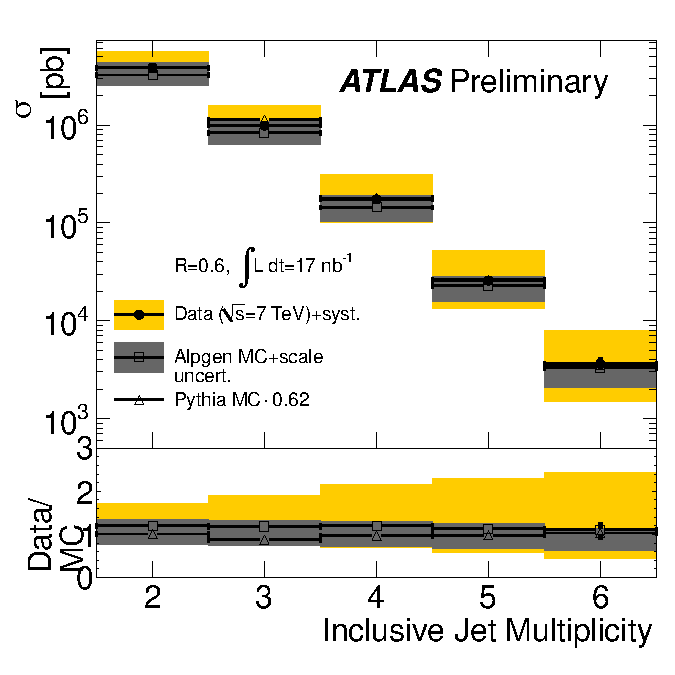
\includegraphics[width=\linewidth,height=\textheight,keepaspectratio]{background/multijet_rates}
        \caption{
            Production cross-section as a function of jet number\cite{multijet_measurement}.
            This measurement was made at a CoM energy of 7 TeV and used an \antikt $\Rparam$-parameter of 0.6.
        }
        \label{fig:multijet_rates}
    \end{figure}

    For the \vbfproc process, the background consists mostly of QCD multijet events,
        with a smaller portion of \ttbar events.
    The usual approach of simulating the background using Monte-Carlo techniques is not feasible,
        as such simulations are inaccurate when trying to model such complex many-jet processes,
        and take far too long to generate at the necessary scale.
    Instead, the yield from background in the SR data is predicted based on the background yield in the Control Regions of the data.
        
    The fundamental assumption for this data-driven background estimate
        is that background events with only two b-tagged jets (2b data)
        will have kinematics very similar to the background events with 4 b-tagged (4b) jets.
    Thus, the kinematic distribution of the 2b signal region can be used as an estimate of the background in the 4b signal region.
    Unfortunately, observation of the Control Regions shows that the kinematics of the 2b and 4b data do not match as well as hypothesized.
    As such, the 2b signal data must undergo a ``reweighting'' process,
        which adjusts the kinematic distribution to match that of 4b.
    This reweighting takes the form of a function $R$,
        which for each event $i$ takes a series of kinematic variables $x_i$ as an argument,
        and returns a reweighting value $r_i$ which scales that event's contribution to the kinematic distributions:
        $r_i = R(x_i)$.
    Deriving this function, and determining the appropriate inputs for it,
        are the challenges addressed in the following sections.

\FloatBarrier
\section{Neural Network Training and Uncertainty} \label{sec:nn_training}

    The reweighting function is derived using machine learning techniques (refer back to Section \ref{sec:ml_techniques}).
    A neural network (NN) is trained via the Keras python library\cite{keras} to identify how to reweight 2b data
        such that the cumulative kinematic distribution looks like that of 4b data.
    In order to improve stability in the reweighting function,
        an ensemble of 100 networks (referred to as the ``bootstrap networks'') is trained,
        and the mean of their calculations is used (called the ``Nominal Estimate'').
    Each neural network instance $j$ produces its own per-event reweighting factors $r_{ij}$
        along with a normalization factor $\alpha_j$ associated with it.
    This normalization factor is calculated so the total yield of all 2b reweighted events matches that of the 4b yield in the same region. 
    So for $N$ total 2b events and $N'$ total 4b events, a normalization factor $\alpha_j$ is set such that:
        \begin{equation}
            \sum_{i=1}^{N} \alpha_j r_{ij} = N'
            \quad.
        \end{equation}

    The nominal estimate $\tilde{r}$ constructed from the mean of these networks will not necessarily satisfy this same relation,
        so it is given its own separate normalization $\tilde \alpha$:
        \begin{equation}
            \sum_{i=1}^{N} \tilde \alpha \tilde r_i = N'
            \quad.
        \end{equation}

    \begin{figure}[!htbp]
        \begin{subfigure}{0.48\textwidth}
            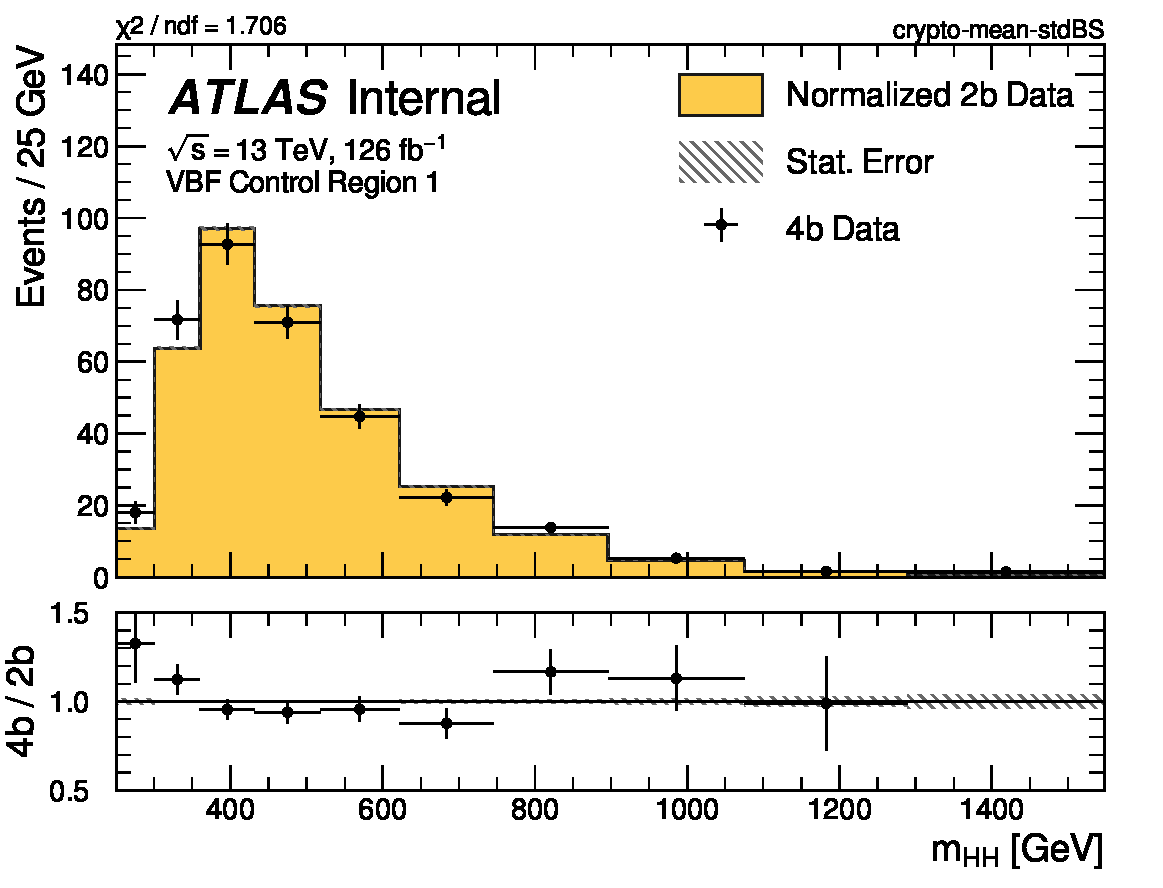
\includegraphics[width=\linewidth,height=\textheight,keepaspectratio]
                {background/crypto-mean-stdBS-m-hh-Control-Region-1-no-rw-all-4binclusive}
            \captionsetup{justification=centering} \caption{Data before reweighting}
        \end{subfigure}
        \begin{subfigure}{0.48\textwidth}
            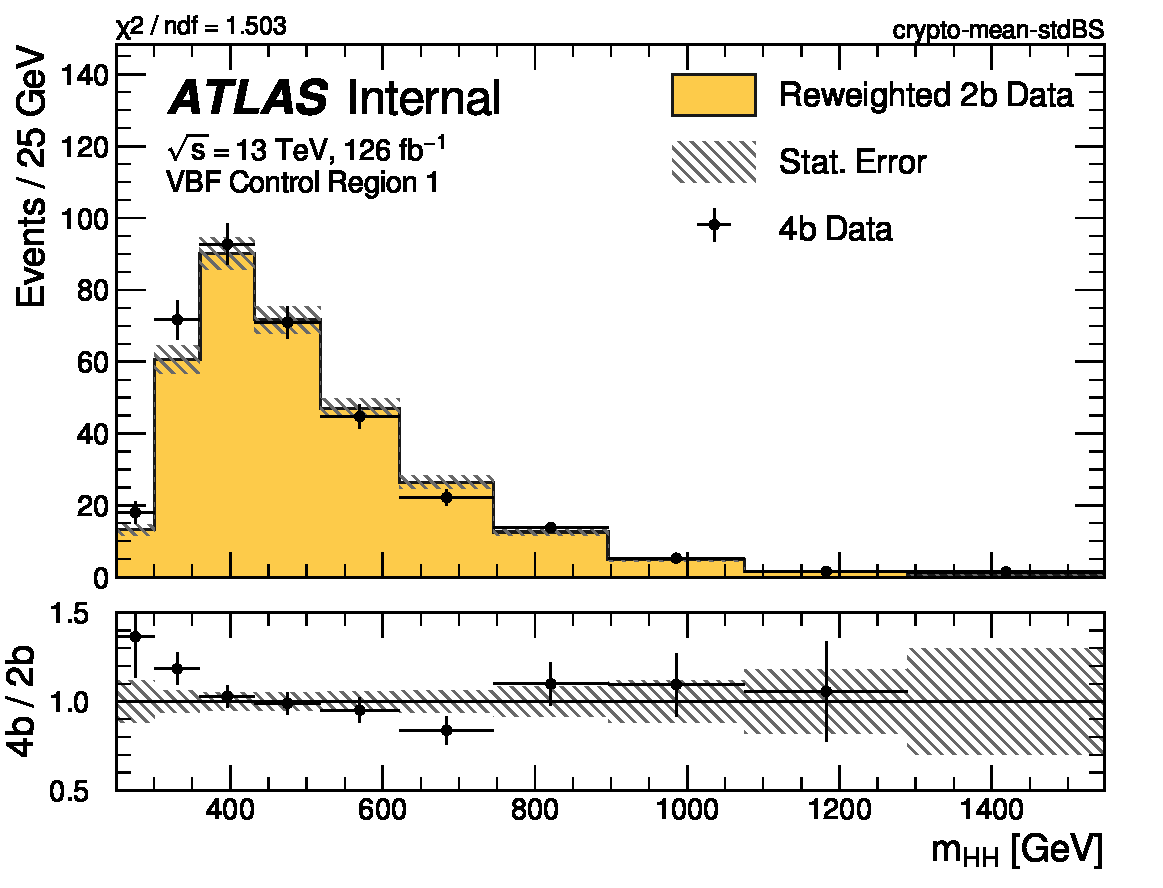
\includegraphics[width=\linewidth,height=\textheight,keepaspectratio]
                {background/crypto-mean-stdBS-m-hh-Control-Region-1-NN-all-4binclusive}
            \captionsetup{justification=centering} \caption{Data after reweighting}
        \end{subfigure}
        \caption{
            The \mhh kinematic distribution of the 2b vs 4b regions, before and after reweighting the 2b region.
        }
        \label{fig:data_mhh_reweight}
    \end{figure}

    \begin{figure}[!htbp]
        \begin{subfigure}{0.48\textwidth}
            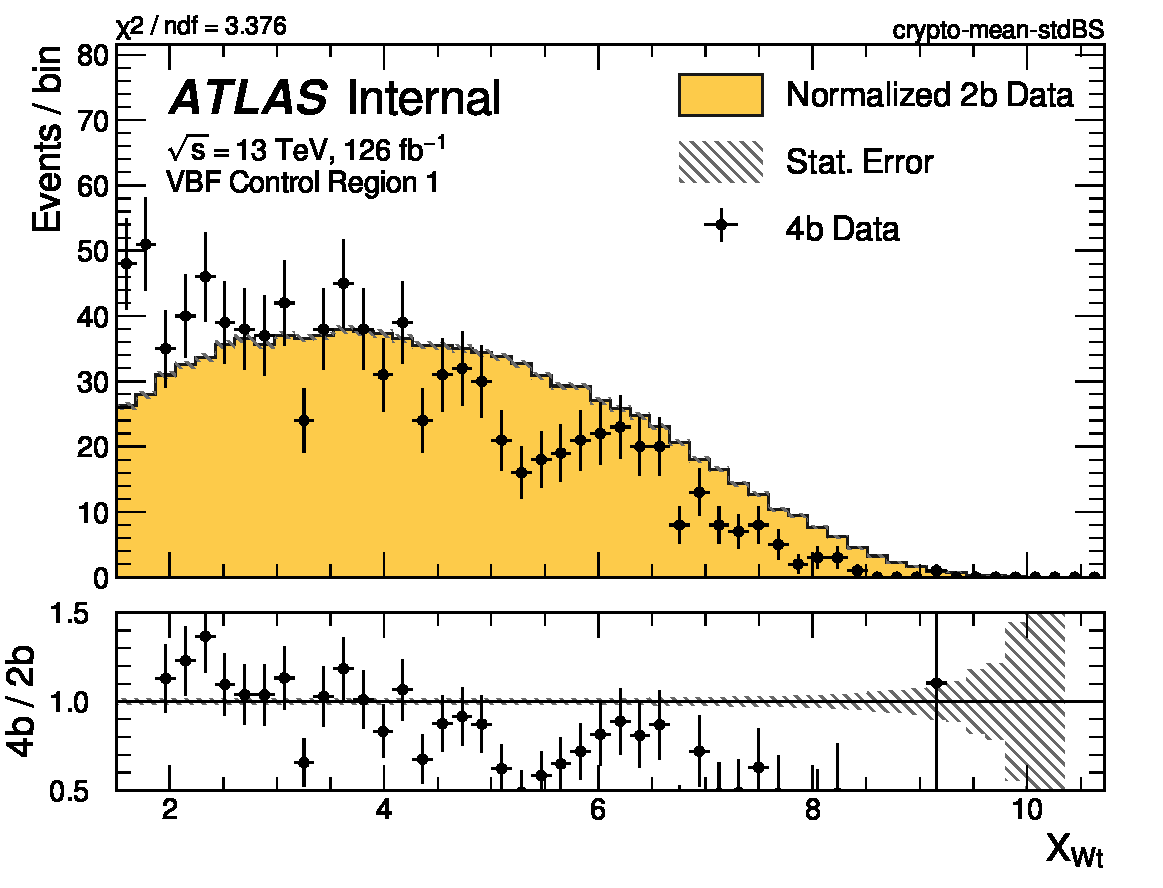
\includegraphics[width=\linewidth,height=\textheight,keepaspectratio]
                {background/crypto-mean-stdBS-X-wt-tag-Control-Region-1-no-rw-all-4binclusive}
            \captionsetup{justification=centering} \caption{Data before reweighting}
        \end{subfigure}
        \begin{subfigure}{0.48\textwidth}
            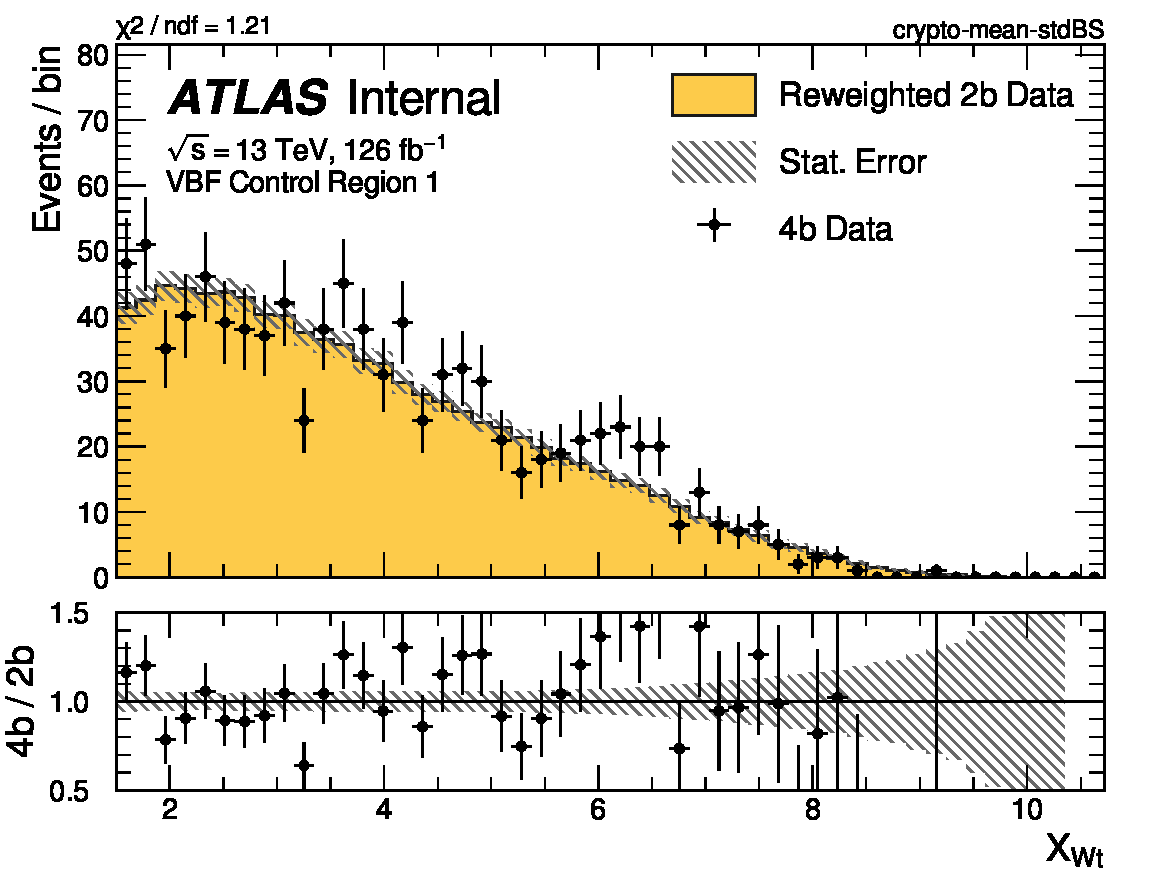
\includegraphics[width=\linewidth,height=\textheight,keepaspectratio]
                {background/crypto-mean-stdBS-X-wt-tag-Control-Region-1-NN-all-4binclusive}
            \captionsetup{justification=centering} \caption{Data after reweighting}
        \end{subfigure}
        \caption{
            The Xwt-tag kinematic distribution of the 2b vs 4b regions, before and after reweighting the 2b region.
        }
        \label{fig:data_xwt_reweight}
    \end{figure}

    \begin{figure}[!htbp]
        \begin{subfigure}{0.48\textwidth}
            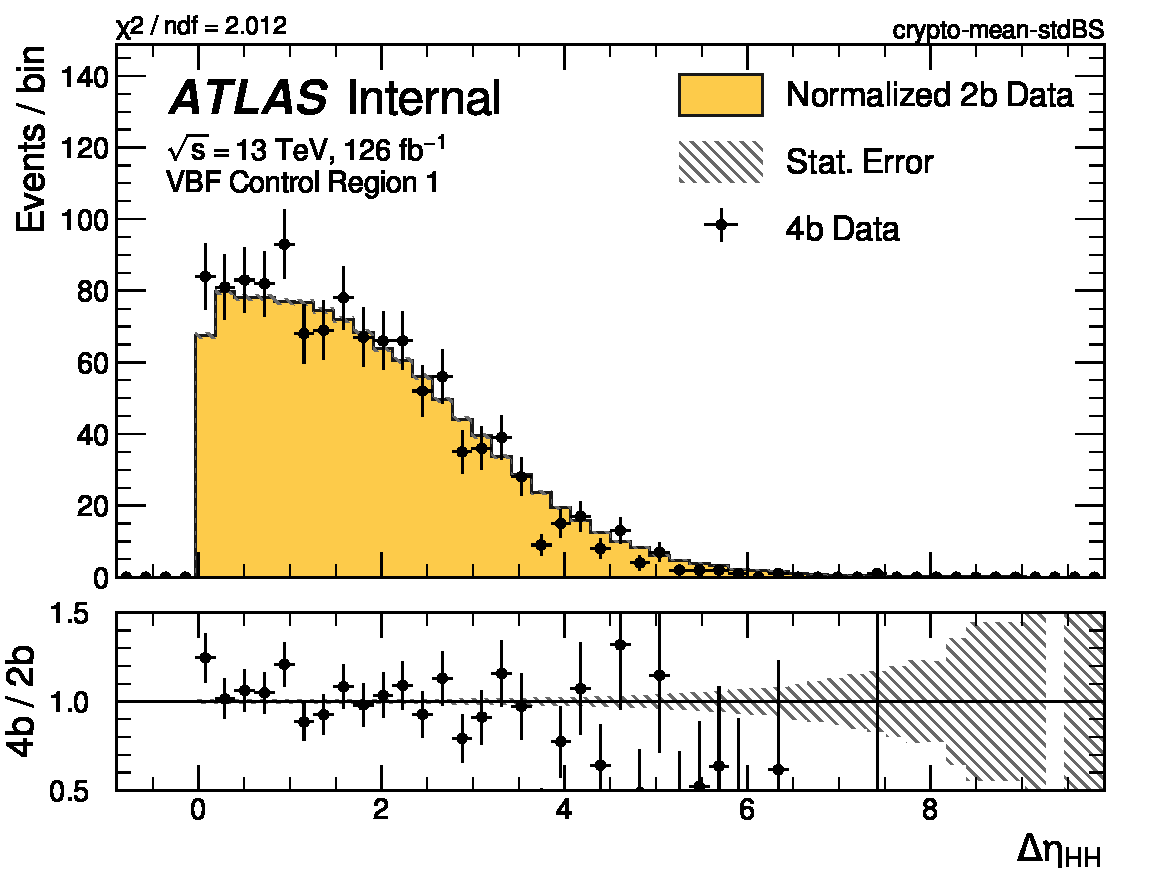
\includegraphics[width=\linewidth,height=\textheight,keepaspectratio]
                {background/crypto-mean-stdBS-dEta-hh-Control-Region-1-no-rw-all-4binclusive}
            \captionsetup{justification=centering} \caption{Data before reweighting}
        \end{subfigure}
        \begin{subfigure}{0.48\textwidth}
            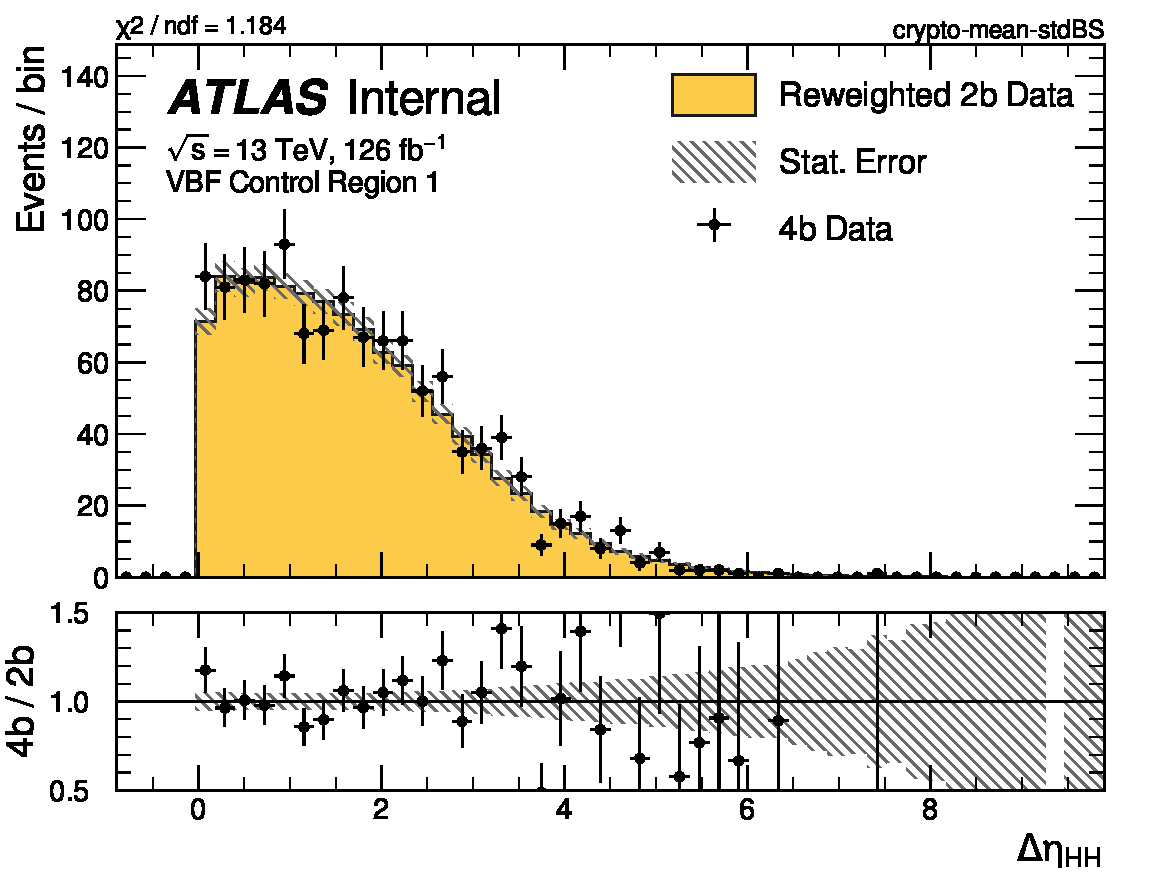
\includegraphics[width=\linewidth,height=\textheight,keepaspectratio]
                {background/crypto-mean-stdBS-dEta-hh-Control-Region-1-NN-all-4binclusive}
            \captionsetup{justification=centering} \caption{Data after reweighting}
        \end{subfigure}
        \caption{
            The $\deta_{HH}$ kinematic distribution of the 2b vs 4b regions, before and after reweighting the 2b region.
        }
        \label{fig:data_detahh_reweight}
    \end{figure}

    The problem with this training approach is that the 4b signal region cannot be used in the training.
    Instead, the neural networks are trained using the CR1 data
        and are optimized to reweight the 2b CR1 data to resemble the 4b CR1 data.
    Because the reweighting function is trained on a different kinematic region than the signal region,
        there is a potential systematic uncertainty that must be assessed.
    This is calculated by training a different ensemble of NNs on CR2.

    \begin{figure}[tbh]
        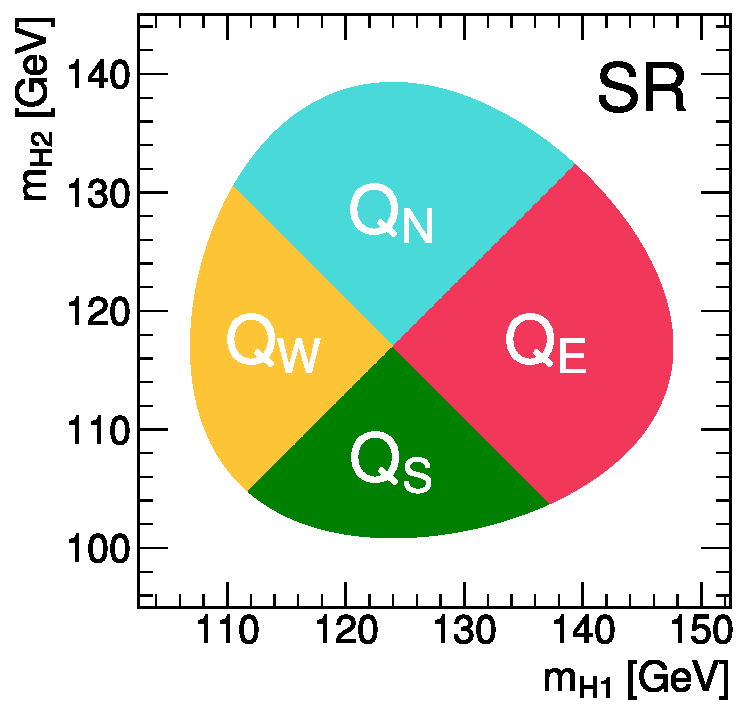
\includegraphics[width=\linewidth,height=\textheight,keepaspectratio]{background/quadNP_viz}
        \caption{
            The Signal Region quadrant splitting used for calculating systematic uncertainties on the background estimate.
            The angles of the split are set to match the angle found in Fig. \ref{fig:region_definition}.
            The four regions are named after the cardinal directions (North, East, South, West)
                to which they correspond on this plot.
        }
        \label{fig:sig_quads}
    \end{figure}

    As seen in Fig. \ref{fig:sig_quads}, the signal region is split into four quadrants,
        with the divisions angled to match those of CR1 and CR2.
    The nominal reweighting is performed using the entire signal region,
        with the events binned by their \mhh value to form a nominal histogram.
    Four alternate histograms are then generated from events reweighted using
        \textit{both} the CR1-trained NN and the CR2-trained NN.
    Specifically, for each of these alternate histograms,
        events from three out of the four signal region quadrants will be reweighted using the CR1 NN.
    The events from the fourth quadrant are reweighted via the CR2 NN.
    A bin-by-bin (absolute) difference between the nominal histogram and each of the alternate histograms 
        is then used to produce the four systematic ``shape'' uncertainties.

    \begin{figure}[tbh]
        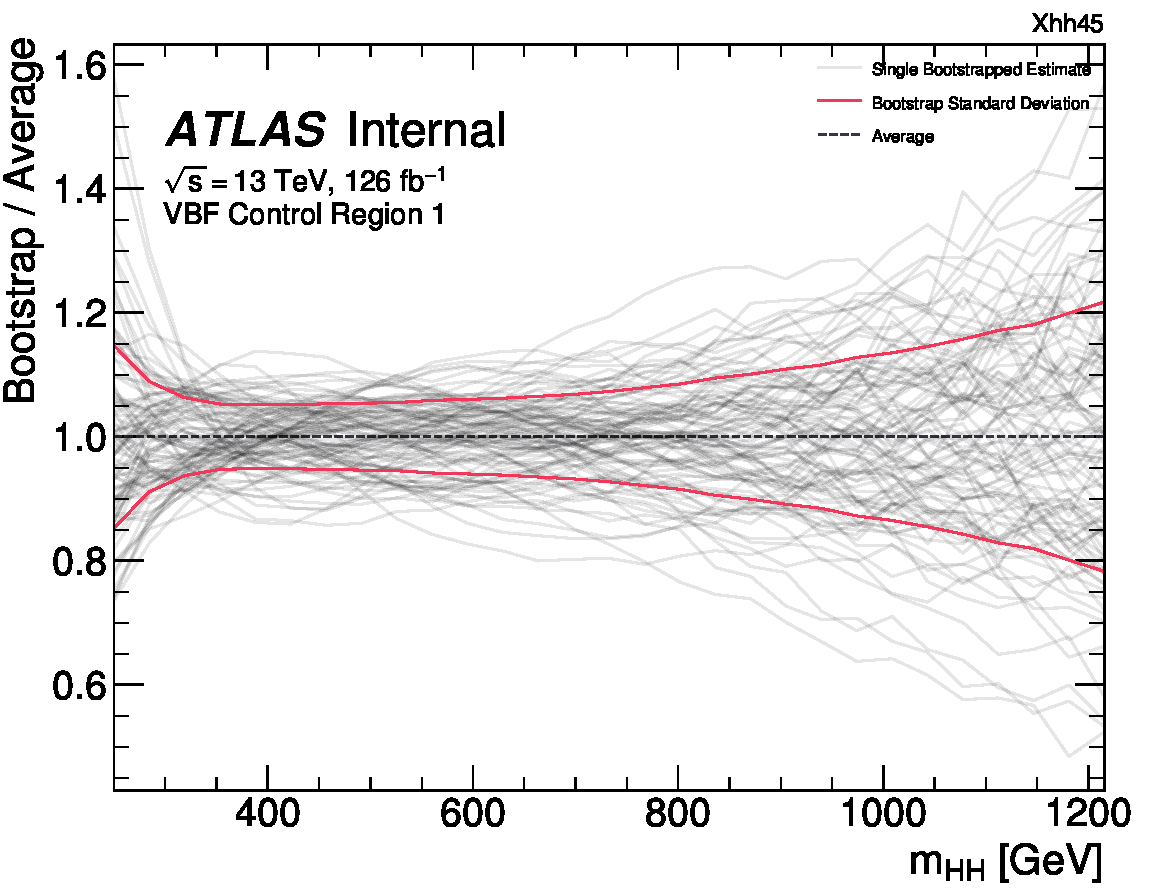
\includegraphics[width=\linewidth,height=\textheight,keepaspectratio]{background/spider-VBF-stdev-Xhh45-m-hh-control-all-4b}
        \caption{
            A diagram illustrating the bootstrap uncertainty for the background estimation neural network.
            The thin gray lines each correspond to the \mhh histogram of one of the 100 bootstrap networks.
            Each of their bins is expressed here as a ratio to their collective average (the dashed line).
            The standard deviation at each bin is then shown with the red lines,
                which can be seen to perform well in expressing the overall behavior
                of the individual bootstraps' deviations from the average.
        }
        \label{fig:spider}
    \end{figure}

    In addition to the systematic shape uncertainty,
        an additional statistical ``bootstrap'' uncertainty is calculated to account for the variation of the bootstrap neural networks.
    This uncertainty is calculated by producing an \mhh histogram for each of the 100 bootstrap NNs.
    The standard deviation of each bin across all 100 bootstrap histograms is calculated,
        and then assigned as a statistical error for that bin of the nominal histogram (see Fig. \ref{fig:spider}).
    This statistical error is treated as a true \textit{statistical} error
        (not systematic, like the shape uncertainties)
        and is ultimately added in quadrature with the standard yield-based statistical uncertainty
        in the background estimate.


\FloatBarrier
\section{VBF Background Reweighting Variables} \label{sec:vbf_bgdNNRW}

    The Neural Network used to reweight the 2b-Tagged CR1 data into the 4b Signal region
        uses a different set of variables when trained for the VBF process than it does for ggF.
    This list of variables was selected through two correlation tests,
        the first of which was determining how strongly correlated different variables are to \mhh
        (Figs. \ref{fig:mhh_corrLT1.5} and \ref{fig:mhh_corrGT1.5}).
    I used the Pearson correlation coefficient as a measure of the relationship of different variables.
    This coefficient $\rho$ is a scalar metric of how closely
        two variables $x$ and $y$ follow a linear correlation, measured as
        \begin{equation}
            \rho_{xy} \equiv \frac{\textrm{cov}(x,y)}{\sigma_x \sigma_y}
            \,.
        \end{equation}
    This is a function of the standard deviations $\sigma_x,\sigma_y$ of $x$ and $y$,
        as well as their \textit{covariance} 
        $\textrm{cov}(x,y) \equiv \overline{(x-\bar{x})(y-\bar{y})}$
        (with $\bar{f}$ being the expectation value of $f$)\cite{pearson_correlation}.


    %\resizebox{0.9\textwidth}{!}{
    \begin{sidewaysfigure}[tbh]
        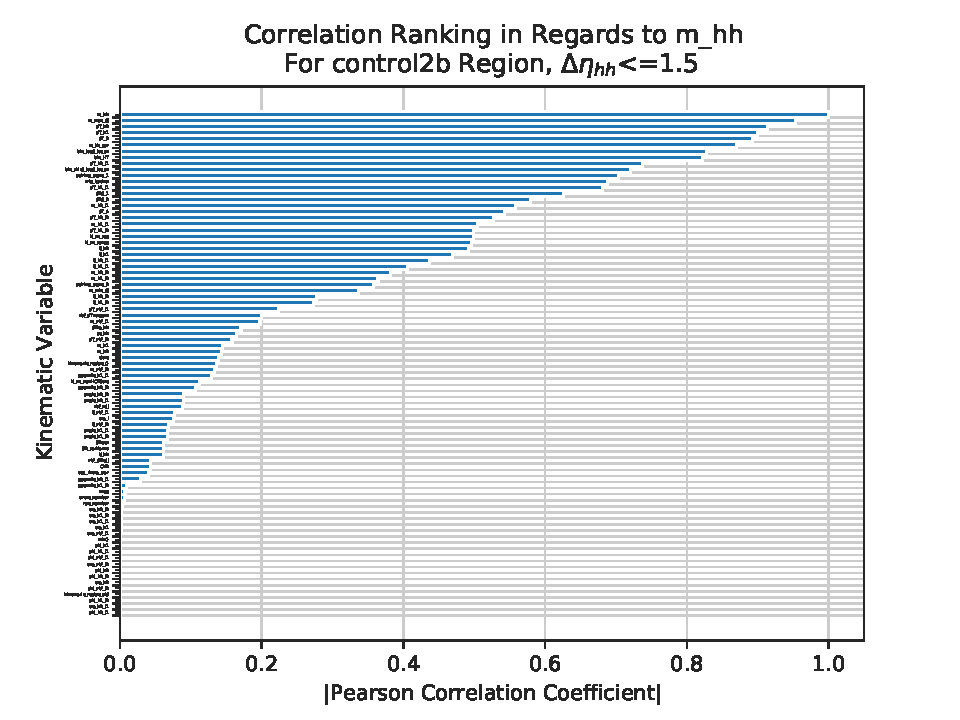
\includegraphics[width=0.9\linewidth,height=\textheight,keepaspectratio]{background/correlation_control2b_detahh-LTE1p5_hist_m_hh}
        \caption{
            The Pearson Correlation Coefficients associated with \mhh for the 2b CR1 data,
                with $\deta \leq 1.5$.
            The higher up on the chart a variable is, the more strongly correlated it is to \mhh,
                with \mhh itself at the top with a coefficient of 1.
            Note that most of the VBF-specific variables, such as vbf\_mjj, are very poorly correlated to \mhh and thus not preferred.
        }
        \label{fig:mhh_corrLT1.5}
    \end{sidewaysfigure}
    %}

    \begin{sidewaysfigure}[tbh]
        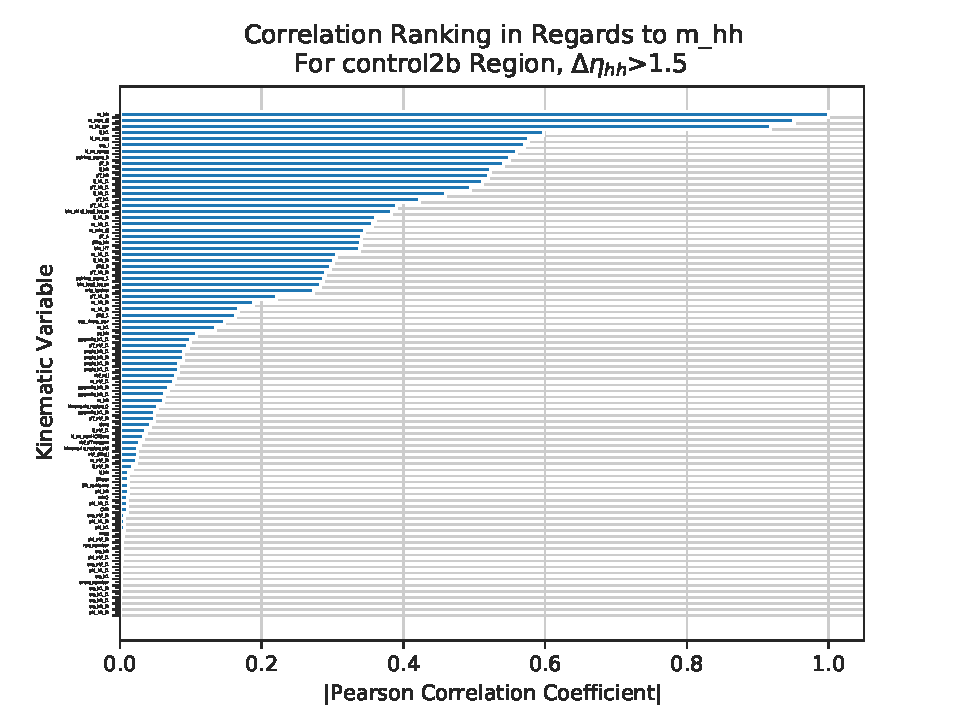
\includegraphics[width=0.9\linewidth,height=\textheight,keepaspectratio]{background/correlation_control2b_detahh-GT1p5_hist_m_hh}
        \caption{
            The Pearson Correlation Coefficients associated with \mhh for the 2b CR1 data,
                with $\deta > 1.5$.
            The higher up on the chart a variable is, the more strongly correlated it is to \mhh,
                with \mhh itself at the top with a coefficient of 1.
            Note that most of the VBF-specific variables, such as vbf\_mjj, are very poorly correlated to \mhh and thus not preferred.
        }
        \label{fig:mhh_corrGT1.5}
    \end{sidewaysfigure}

    Based on their high correlation to \mhh in both \deta regions, 23 variables were then selected for further study.
    These 23 variables were plotted against each other in a correlation matrix,
        which displayed the dependence of each variable on the others.
    A final set of seven variables was selected based (Table \ref{tab:vbf_NNRW_vars}) on which variables were \textit{least} correlated to each other,
        in order to avoid variables carrying redundant information (Figs. \ref{fig:vbf_corr_matrix_LT1.5} and \ref{fig:vbf_corr_matrix_GT1.5}).
    The culmination of this work is a neural network well suited to modelling the background process of the analysis.
    All that remains before the final ATLAS data can be analyzed then,
        is a suitable modelling of the signal process itself.

    \begin{figure}[tbh]
        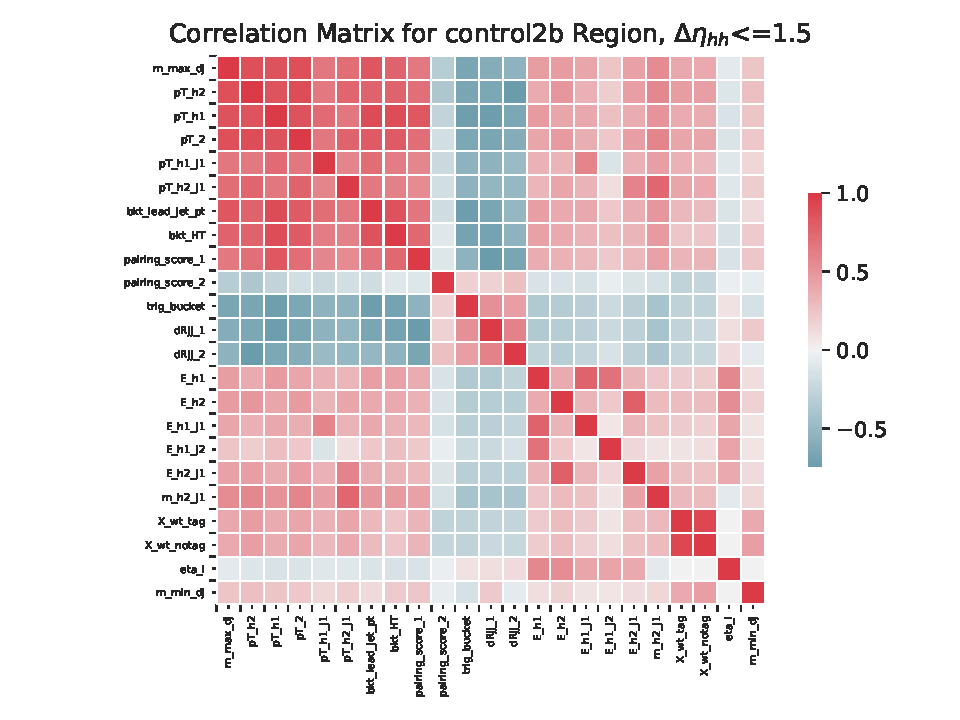
\includegraphics[width=\linewidth,height=\textheight,keepaspectratio]{background/correlation_control2b_detahh-LTE1p5_matrix}
        \caption{
            The Pearson Correlation Coefficients matrix associated with variables in the 2b Control Region data,
                with $\deta \leq 1.5$.
            Bins with more saturated (i.e.\ more blue or more red) colors indicate strong correlation between those two variables.
            All variables are of course 100\% correlated to themselves, hence the deep red line running down the diagonal.
            The most highly preferred variables are those with correlation coefficients near 0 for as many other variables as possible.
            If a variable (i.e.\ m\_max\_dj) is selected, any other variables with strong correlations to it (i.e.\ pT\_h2)
                are then strongly disfavored for later selection.
        }
        \label{fig:vbf_corr_matrix_LT1.5}
    \end{figure}

    \begin{figure}[tbh]
        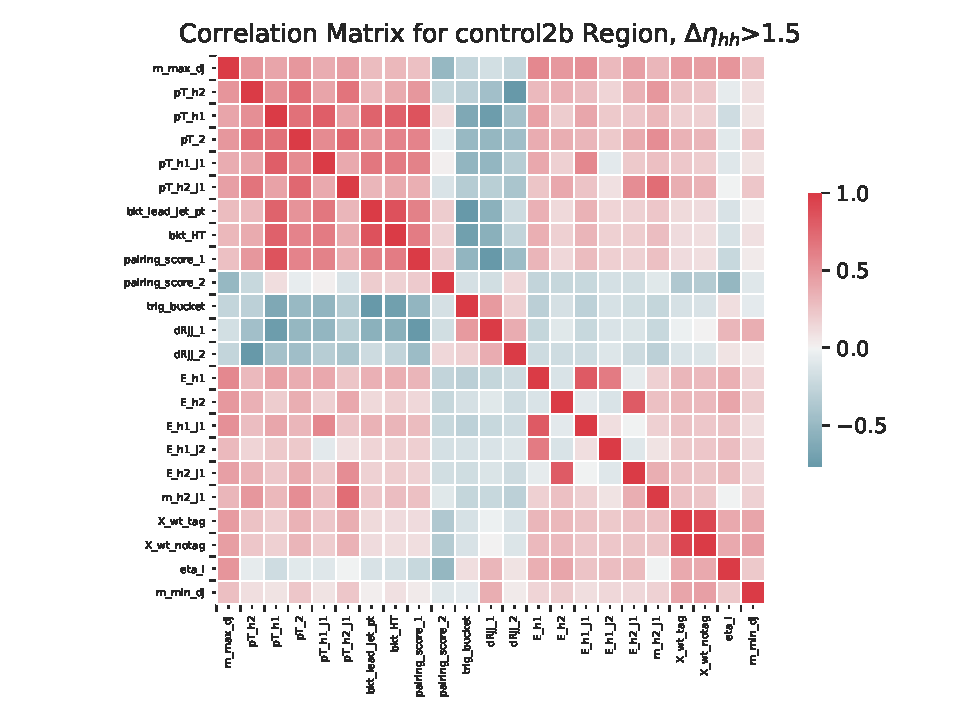
\includegraphics[width=\linewidth,height=\textheight,keepaspectratio]{background/correlation_control2b_detahh-GT1p5_matrix}
        \caption{
            The Pearson Correlation Coefficients matrix associated with variables in the 2b Control Region data,
                with $\deta > 1.5$.
            Bins with more saturated (i.e.\ more blue or more red) colors indicate strong correlation between those two variables.
            All variables are of course 100\% correlated to themselves, hence the deep red line running down the diagonal.
            The most highly preferred variables are those with correlation coefficients near 0 for as many other variables as possible.
            If a variable (i.e.\ m\_max\_dj) is selected, any other variables with strong correlations to it (i.e.\ pT\_h2)
                are then strongly disfavored for later selection.
        }
        \label{fig:vbf_corr_matrix_GT1.5}
    \end{figure}


    \begin{table}[!htbp] \centering \scriptsize
    \caption{Final Set of Neural Network Variables.}
    \label{tab:vbf_NNRW_vars}
    \begin{tabular}{ |l|l|l| }
        \hline
        \textbf {Variable} & \textbf {Internal Name} & \textbf {Description} \\
        \hline
        $M_{max \Delta j}$ & \code{m\_max\_dj}         & 
            Take the di-jet mass of the six possible pairings\\
            && of the four higgs’ candidate jets;\\
            && this is the maximum di-jet mass of those pairings \\ 
        \hline
        $M_{min \Delta j}$ & \code{m\_min\_dj}         & 
            As above, but the minimum \\
        \hline
        $E_{H1}$           & \code{E\_h1}              & 
            Energy of the leading-$p_T$ reconstructed Higgs \\
        \hline
        $E_{H2}$           & \code{E\_h2}              & 
            Energy of the sub-leading-$p_T$ reconstructed Higgs \\
        \hline
        Xwt-tag            & \code{X\_wt\_tag}         & 
            $\log\left(X_{Wt}\right)$, where $X_{Wt}$ is the variable used for the top veto \\
        \hline
        $\eta_i$           & \code{eta\_i}             & 
            Average $\eta$ of the four Higgs decay jets \\
        \hline
        Pairing Score 2    & \code{pairing\_score\_2 } & 
            This changes depending on the Higgs pairing algorithm used. \\
            &&The current algorithm used is minDR. \\
            &&With four jets, there are three possible pairings of the jets. \\
            &&The pairings are ranked by the $\Delta R$ of the leading-$p_T$ Higgs candidate. \\
            &&Pairing Score 2 is the $\Delta R$ of the second-smallest of these pairings. \\
        \hline
    \end{tabular} \end{table}
